\appendix

\section{Matrix operations}
\subsection{Skew Symmetric Matrix}
A skew-symmetric matrix is a matrix where $A^\top=-A$\\
$[\cdot]^\times$ is the skew-symmetric operator and is applied to turn vectors into skew-symmetric matrices.

Example:\\
Let $u=[u_1,u_2,u_3]^\top$, then:
$$
u^\times=\begin{bmatrix}
0 & -u_3 & u_2 \\ u_3 & 0 & -u_1 \\ -u_2 & u_1 & 0
\end{bmatrix}
$$
The skew-symmetric operator has the following relation to the cross-product:
$$
u^\times v=u\times v
$$

\subsection{Cross-Product}
The cross-product between two $3\times1$ vectors $a$ and $b$ is defined as:
$$
a\times b = \det
\begin{pmatrix}
\vec{i} & \vec{j} & \vec k \\ a_1  & a_2  & a_3 \\ b_1 & b_2 & b_3
\end{pmatrix}
$$

\subsection{Matrix Calculus}

\subsubsection{Partial Derivative (Jacobian)}
Let
$$
f(x)= 
\begin{bmatrix}
f_1(x) \\  f_2(x) \\ \vdots \\ f_n(x)
\end{bmatrix}
, x\in \mathbb{R}^m
$$
Then the Jacobian of $f$ is given by
$$
\frac{\partial f}{\partial x}=
\begin{bmatrix}
\frac{\partial f}{\partial x_1} & \frac{\partial f}{\partial x_2} & \cdots & \frac{\partial f}{\partial x_m}
\end{bmatrix}
$$

The Jacobian of the vector function $f(x) = Ax$ is
$$
\frac{\partial}{\partial x}(Ax)=A
$$

\subsubsection{Chain Rule}
$$
\frac{\partial \mathrm{f}(\mathrm{g}(\mathrm{x}))}{\partial \mathrm{x}}=\left.\frac{\partial \mathrm{f}(\mathrm{y})}{\partial \mathrm{y}}\right|_{\mathrm{y}=\mathrm{g}(\mathrm{x})} \frac{\partial \mathrm{g}(\mathrm{x})}{\partial \mathrm{x}}
$$
\subsubsection{Full derivative}
(From lecture notes)
Consider a function:
$$
f(x, y)
$$
where $\mathrm{y}=\mathrm{g}(\mathrm{x})$. Then the partial derivative ignores that $\mathrm{y}$ is intrinsically a function of x, i.e.
$$
\frac{\partial \mathrm{f}(\mathrm{x}, \mathrm{y})}{\partial \mathrm{x}}
$$
disregards this dependency, while the total derivative takes it into account and does:
$$
\frac{\mathrm{df}(\mathrm{x}, \mathrm{y})}{\mathrm{dx}}=\frac{\partial \mathrm{f}(\mathrm{x}, \mathrm{y})}{\partial \mathrm{x}}+\frac{\partial \mathrm{f}(\mathrm{x}, \mathrm{y})}{\partial \mathrm{y}} \frac{\partial \mathrm{y}}{\partial \mathrm{x}}=\frac{\partial \mathrm{f}(\mathrm{x}, \mathrm{y})}{\partial \mathrm{x}}+\frac{\partial \mathrm{f}(\mathrm{x}, \mathrm{y})}{\partial \mathrm{y}} \frac{\partial \mathrm{g}}{\partial \mathrm{x}}
$$

\subsubsection{Gradient}
The gradient is an operator where you can differentiate \textbf{scalar} functions w.r.t. vectors. Let $f(x)$ be a scalar function of the vector $x$ i.e. $f:\mathbb R^n\rightarrow\mathbb R$, then
$$
\nabla f(x)=\left[\frac{\partial f}{\partial x}\right]^\top=
\begin{bmatrix}
    \frac{\partial f}{\partial x_1}\\
    \vdots\\
    \frac{\partial f}{\partial x_n}
\end{bmatrix}
$$

For the linear function $f(x)=c^\top x=x^\top c$, we have
\begin{equation*}
    \begin{split}
        \nabla(c^\top x)=c\\
        \nabla(x^\top c)=c\\
    \end{split}
\end{equation*}

The gradient of the quadratic function $f(x) = \frac{1}{2}x^\top Gx$ is
$$
\nabla f(x) = \frac{1}{2}Gx + \frac{1}{2}G^\top x
$$
or, when $G$ is a symmetric matrix:
$$
\nabla f(x) = Gx,\quad G = G^\top
$$
\subsubsection{Matrix differentiation}
\begin{equation*}
    \begin{split}
        \frac{\partial }{\partial X}\text{tr}(XA)&=A^\top\\
        \frac{\partial }{\partial X}\text{tr}(AX^\top)&=A\\
        \frac{\partial }{\partial X}\text{tr}(XAX^\top)&=XA^\top+XA
    \end{split}
\end{equation*}
where $X$ and $A$ are matrices and $\text{tr}(\cdot)$ is the trace operator (sum of the diagonal elements).

\section{Matrix properties}

\subsection{Eigenvalues}
\begin{align}
    \begin{split}
        Av &= \lambda v
        \\
        (A-\lambda I)v &= 0
        \\
        \textbf{Det}(A-\lambda I) &= 0
    \end{split}
\end{align}

\subsection{Invertible matrices}
If a matrix $\mathbf{A}$ is invertible, equivalent terms are:
\begin{itemize}
    \item $\mathbf{A}$ has full rank
    \item $\mathbf{A}$ is rank efficient
    \item $\textbf{Det}(A)$ is non-zero
    \item $\mathbf{A}$ is non-singular
\end{itemize}

\subsection{Symmetry}
A matrix $\mathbf{A}$ is symmetric if,
\begin{equation}
    A = A^\top 
\end{equation}

\textbf{Note:} All diagonal matrices are symmetric.

\subsection{Positive definiteness}
A matrix $\mathbf{A}$ is positive definite if,
\begin{itemize}
    \item $\mathbf{x^\top A x} > 0$, and semi-definite if $\mathbf{x^\top A x} \geq 0$ for all $\mathbf{x} \neq \mathbf{0}$
    \item All principle minors have eigenvalues $\lambda > 0$. Each principle minor is a sub-matrix of $\textbf{A}$ which has reduced number of column and rows from original $\textbf{A}$ matrix.
\end{itemize}

\section{Vector operations}

\subsection{Norms}
\begin{align}
    \begin{split}
        \mathbf{x}& = \begin{bmatrix}
            x_1 \\ \vdots \\ x_n
        \end{bmatrix}
        \\
        ||\mathbf{x}&|| = ||\mathbf{x}||_2 = \sqrt{\mathbf{x}^\top \mathbf{x}} = \sqrt{\sum_{i=1}^n x_i^2}
        \\
        ||\mathbf{x}&||_1 = \sum_{i=1}^n |x_i|
        \\
        ||\mathbf{x}&||_\infty = \max_k |x_k|
    \end{split}
\end{align}

\subsection{Scalar Product}
\begin{align}
    \begin{split}
        \mathbf{x^\top y} \quad \mathbf{x, y} \in \mathcal{R}^n
    \end{split}
\end{align}

\subsection{Cross product derivative}

\begin{equation}
    \frac{d}{dt} \Vec{a} \times \Vec{b} = \frac{d\Vec{a}}{dt} \times \Vec{b} + \Vec{a} \times \frac{d\Vec{b}}{dt}
\end{equation}

\section{Vector notation conventions}

Equation \ref{eq:vector_conv} shows the vector from point $x$ to point $y$ given in frame $b$.

\begin{equation}
\label{eq:vector_conv}
    r^b_{xy} = r^b_y - r^b_x
\end{equation} 

Equation \ref{eq:MOI} shows the moment of inertia (MOI) of body $b$ about point $c$ as expressed in frame $a$. Come from pg. 274 eq. (7.73) and (7.74) in book. Where $r^b_i$ is the vector from point $c$ to point $i$.

\begin{equation}
\label{eq:MOI}
    M^a_{b/c} = \sum\limits_{i} -m_i(r^b_i)^\times(r^b_i)^\times = \sum\limits_{i}[(r^b_i)^Tr^b_iI-r^b_i(r^b_i)^T]
\end{equation} 

Equation \ref{eq:w_conv} shows the angular velocity, where $\omega^a_{ab}$ denotes angular velocity of rotation of frame $b$ around $a$ given in $a$'s frame,

\begin{equation}
\label{eq:w_conv}
    \omega^a_{ab} = \omega^b_{??} = -\omega^a_{??} = -\omega^b_{??}
\end{equation} 


where $\omega^a_{ab}$ is angular velocity of frame $b$ relative to frame $a$ in $a$'s coordinate form.
%The $ab$ part accounts for the offset of origin of frame $b$ from $a$, thus the vector only signify the rotation vector pointing out from $b$'s origin expressed in $a$'s coords.

\section{Other formulas}

\subsection{Coordinates}

\subsubsection{Polar Coordinates}

\begin{equation}
\begin{aligned}
    x = r sin\theta cos \phi \\
    y = r sin\theta sin \phi \\
    z = r cos\theta
\end{aligned}
\end{equation}

\begin{figure}[H]
    \centering
    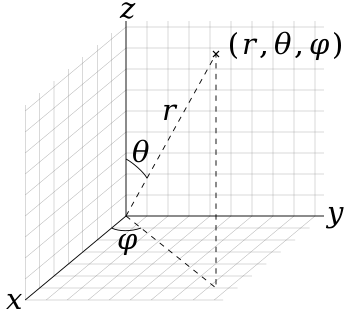
\includegraphics[scale=0.7]{figures/3D_Spherical.svg.png}
    \caption{Polar Coordinates}
    \label{fig:polar}
\end{figure}

\subsection{Linearization}

Consider the system,

\begin{equation}
    \Dot{\mathbf{x}} =  f(\mathbf{x,u}) = \mathbf{Ax + Bu}, \quad \mathbf{y} = h(\mathbf{x}) = \mathbf{Cx + Du}
\end{equation}

It can be linearized by using the part of Taylor including only first derivative,

\begin{equation}
    f(\mathbf{x,u}) \approx \Hat{f}(\mathbf{\Delta x,\Delta u}) = f(\mathbf{x_0,u_0}) + \frac{\partial f}{\partial \mathbf{x}}_{x=x_0, u=u_0} \underbrace{(\mathbf{x - x_0})}_\mathbf{\Delta x} + \frac{\partial f}{\partial \mathbf{u}}_{x=x_0, u=u_0} \underbrace{(\mathbf{u - u_0})}_\mathbf{\Delta u}
\end{equation}

The formula essentially means that after calculating,
the jacobians, we put our former values $\mathbf{x,u}$ as $\mathbf{x_0, u_0}$ in them and the equilibrium point $\mathbf{f(x_0,u_0)}$.


\subsection{Different moments of inertia}

\begin{figure}[H]
    \centering
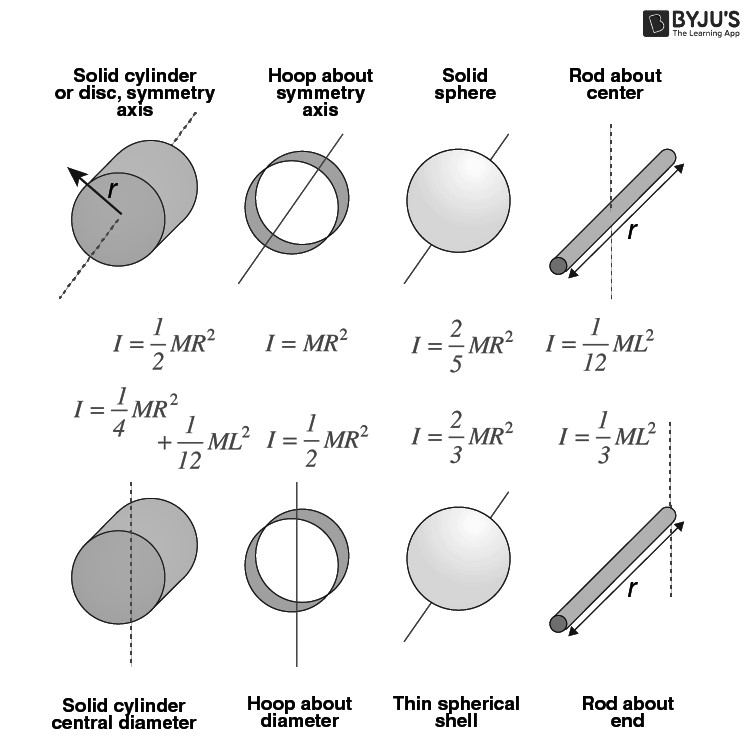
\includegraphics[scale=0.4]{figures/moment of inertia.jpg}
    \caption{Different moments of inertia}
    \label{fig:moments of inertia}
\end{figure}
